%; whizzy section -pdf xpdf -latex ./whizzypdfptex.sh
% latex beamer presentation.
% platex, latex-beamer でコンパイルすることを想定。 

%     Tokyo Debian Meeting resources
%     Copyright (C) 2008 Junichi Uekawa
%     Copyright (C) 2008 Nobuhiro Iwamatsu

%     This program is free software; you can redistribute it and/or modify
%     it under the terms of the GNU General Public License as published by
%     the Free Software Foundation; either version 2 of the License, or
%     (at your option) any later version.

%     This program is distributed in the hope that it will be useful,
%     but WITHOUT ANY WARRANTY; without even the implied warranty of
%     MERCHANTABILITY or FITNESS FOR A PARTICULAR PURPOSE.  See the
%     GNU General Public License for more details.

%     You should have received a copy of the GNU General Public License
%     along with this program; if not, write to the Free Software
%     Foundation, Inc., 51 Franklin St, Fifth Floor, Boston, MA  02110-1301 USA

\documentclass[cjk,dvipdfmx,12pt]{beamer}
\usetheme{Tokyo}
\usepackage{ulem}
\usepackage{tabularx}

\usepackage{fancybox}
\usepackage{fancyvrb}   
\usepackage{float}

% commandline環境を定義。画面入出力についてはcommandline環境
% で表記する
\newenvironment{commandline}%
{\VerbatimEnvironment
  \begin{Sbox}\begin{minipage}{0.9\hsize}\begin{fontsize}{7.3}{7.3} \begin{BVerbatim}}%
{\end{BVerbatim}\end{fontsize}\end{minipage}\end{Sbox}
  \setlength{\fboxsep}{8pt}
% start on a new paragraph

\vspace{6pt}% skip before
\fcolorbox{dancerdarkblue}{dancerlightblue}{\TheSbox}

\vspace{6pt}% skip after
}
%end of commandline

\definecolor{dancerdarkblue}{rgb}{0,0.08,0.45}
\definecolor{dancernormalblue}{rgb}{0.8,0.9,0.95}
\definecolor{dancerlightblue}{rgb}{0.8,0.95,1}


%  preview (shell-command (concat "evince " (replace-regexp-in-string "tex$" "pdf"(buffer-file-name)) "&"))
%  presentation (shell-command (concat "xpdf -fullscreen " (replace-regexp-in-string "tex$" "pdf"(buffer-file-name)) "&"))

%http://www.naney.org/diki/dk/hyperref.html
%日本語EUC系環境の時
\AtBeginDvi{\special{pdf:tounicode EUC-UCS2}}
%シフトJIS系環境の時
%\AtBeginDvi{\special{pdf:tounicode 90ms-RKSJ-UCS2}}

\title{バージョン管理ツールを使い Debian パッケージを管理する}
\subtitle{Git 編}
\author{岩松 信洋 iwamatu@debian.or.jp\\IRC nick: iwamatsu}
\date{2008年4月19日}
\logo{
\includegraphics[width=8cm]{image200607/openlogo-light.eps}}


% 間のタイトルページ用
\newcommand{\emtext}[1]{
\begin{frame}{}
 
\begin{minipage}{0.55\hsize}
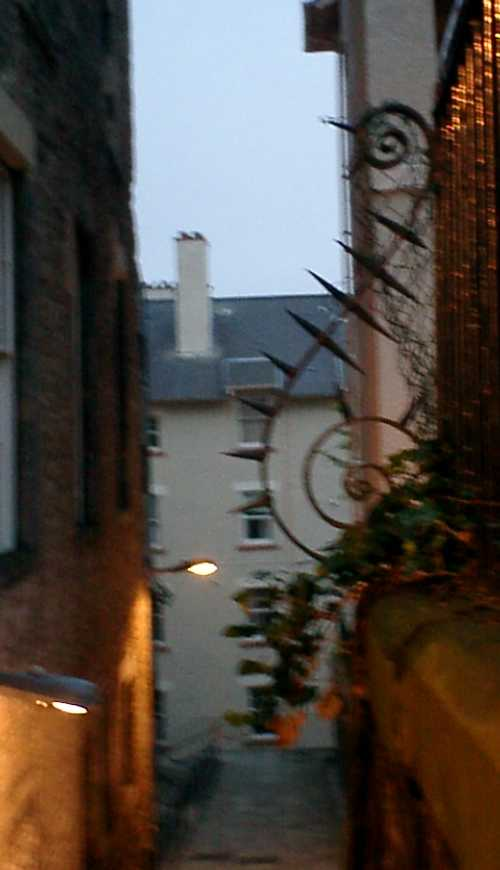
\includegraphics[width=1\hsize]{image200707/gurutitle.jpg}
\end{minipage}
\begin{minipage}{0.39\hsize}
 {\Huge #1
 }
\end{minipage}
\end{frame}
}

% 三択問題用
\newcounter{santakucounter}
\newcommand{\santaku}[5]{%
\addtocounter{santakucounter}{1}
\frame{\frametitle{問題\arabic{santakucounter}. #1}
%問題\arabic{santakucounter}. #1
\begin{minipage}[t]{0.8\hsize}
 \begin{itemize}
 \item
      \begin{minipage}{0.2\hsize}
      
\includegraphics[width=0.9\hsize]{image200703/janken-A.png}\end{minipage} 
       \begin{minipage}{0.6\hsize}
       A #2\end{minipage}\\
 \item
      \begin{minipage}{0.2\hsize}
      
\includegraphics[width=0.9\hsize]{image200703/janken-B.png}\end{minipage} 
       \begin{minipage}{0.6\hsize}
       B #3\end{minipage}\\
 \item
      \begin{minipage}{0.2\hsize}
      
\includegraphics[width=0.9\hsize]{image200703/janken-C.png}\end{minipage} 
       \begin{minipage}{0.6\hsize}
       C #4\end{minipage}\\
 \end{itemize}
\end{minipage}
}
\frame{\frametitle{問題\arabic{santakucounter}. #1}
%問題\arabic{santakucounter}. #1
\begin{minipage}[t]{0.8\hsize}
\begin{itemize}
 \item
      \begin{minipage}{0.2\hsize}
      
\includegraphics[width=0.9\hsize]{image200703/janken-A.png}\end{minipage} 
       \begin{minipage}{0.6\hsize}
       A #2\end{minipage}\\
 \item
      \begin{minipage}{0.2\hsize}
      
\includegraphics[width=0.9\hsize]{image200703/janken-B.png}\end{minipage} 
       \begin{minipage}{0.6\hsize}
       B #3\end{minipage}\\
 \item
      \begin{minipage}{0.2\hsize}
      
\includegraphics[width=0.9\hsize]{image200703/janken-C.png}\end{minipage} 
       \begin{minipage}{0.6\hsize}
       C #4\end{minipage}\\
\end{itemize}
\end{minipage}
\begin{minipage}[t]{0.15\hsize}
答えは:

\vspace{1cm}

  {\huge \hspace{1cm}#5}
  \hspace{-6cm}\includegraphics[width=4cm]{image200703/janken-#5.png}
 \end{minipage}}
}

\begin{document}

\frame{\titlepage{}}


\section{はじめに}

\begin{frame}{なぜパッケージもVCSで管理するのか}
\begin{itemize}
  \item 異なるバージョンのパッケージを管理することができる。
  \item チームでの開発体制を容易に構築できる。
  \item アップストリームとの連携
\end{itemize}
\end{frame}

\begin{frame}{Debian で使用可能な VCS}
\begin{center}
2008年4月の時点での Debian で利用可能な VCS
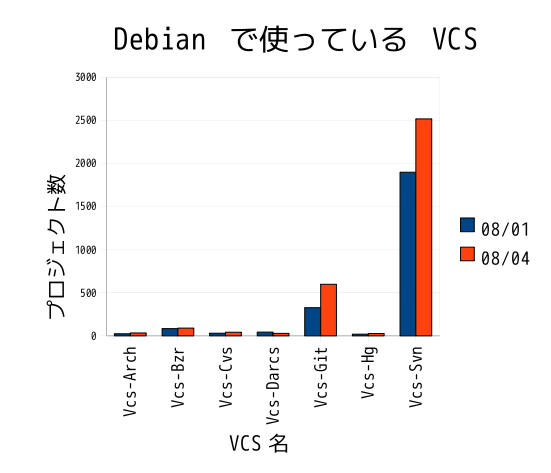
\includegraphics[width=1.0\hsize]{image200804/debian-vcs-200804.png}
\end{center}
\end{frame}


\begin{frame}{git-buildpackage}

\begin{itemize}

\item git-buildpackage 

パッケージを作成する \\
\item git-dch 

Git のコミットログから Debian Changelog を作成する。\\
\item git-import-dsc 

既存の Debian Package をGitにインポートする。\\
\item git-import-orig 

アップストリームからリリースされたソースコードをGitにインポートする。\\

\end{itemize}
\end{frame}

\begin{frame}{Gitの簡単な使い方}
\begin{center}
SD 2008年 4月号 を買うといいよ。
%\includegraphics[width=0.5\hsize]{image200804/1208082175384ed79.jpg}
\end{center}
\end{frame}

\begin{frame}{Gitの簡単な使い方}
   \begin{itemize}
\item git clone

リモートリポジトリから情報を取得し、ローカルリポジトリを作成する。\

\item git init

ローカルリポジトリを作成する。\\
\item git add

ローカルリポジトリのキャッシュ(index)に管理対象のファイルを追加する。\\
\item git commit

ローカルリポジトリに変更を反映する。\\
\item git rm

ローカルリポジトリから管理対象ファイルを削除する。\\
\item git diff

\end{itemize}
\end{frame}

\begin{frame}{Gitの簡単な使い方}
   \begin{itemize}
   \item git diff

差分を取得する。\\
\item git branch

ブランチを作成する。\\
\item git checkout

作成したブランチをチェックアウトする。\\
\item git format-patch

パッチを作成する。\\

\item git pull

リモートリポジトリから変更を取得する。\\

\item git push

リモートリポジトリへ変更を反映する。\\
\end{itemize}
\end{frame}

\emtext{パッケージ化されているものを Git で管理する}

\begin{frame}[containsverbatim]{Debian Package 情報の取り込み}

\begin{minipage}{0.5\hsize}

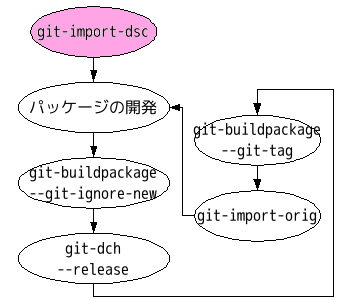
\includegraphics[width=1.0\hsize]{image200804/test1-1.png}
\end{minipage} 
\begin{minipage}{0.45\hsize}
\begin{commandline}
$ git-import-dsc ../isight-firmware-
tools_1\.0.2-1.dsc
Upstream version: 1.0.2
Debian version: 1
No git repository found, creating one.
Initialized empty Git repository in \
.git/
Everything imported under isight-firm\
ware-tools
$ ls
isight-firmware-tools
$ cd isight-firmware-tools
$ git branch
* master
  upstream
\end{commandline}
\end{minipage}
\end{frame}


\begin{frame}[containsverbatim]{インポート時のログ}

\begin{minipage}{0.5\hsize}

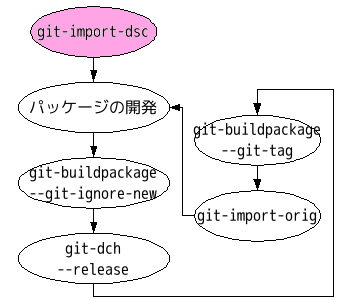
\includegraphics[width=1.0\hsize]{image200804/test1-1.png}
\end{minipage} 
\begin{minipage}{0.45\hsize}
\begin{commandline}
$ git log
commit 9c3669a233afe69d7be2aa8ad199\
5e6b19c841aa
Author: Nobuhiro Iwamatsu <iwamatsu@\
nigauri.org>
Date:   Sun Apr 6 21:48:40 2008 +0900

    Imported Debian patch 1.0.2-1
$ git tag
debian/1.0.2-1
upstream/1.0.2
\end{commandline}
\end{minipage}
\end{frame}
%%

\begin{frame}[containsverbatim]{ソースコードを変更し、修正を管理する}

\begin{minipage}{0.5\hsize}

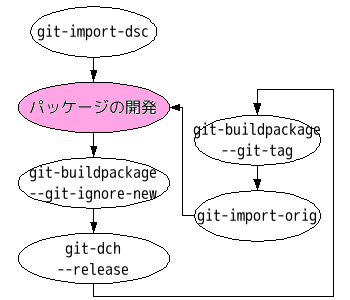
\includegraphics[width=1.0\hsize]{image200804/test1-2.png}
\end{minipage} 
\begin{minipage}{0.45\hsize}

\begin{commandline}
$ dpatch-edit-patch 05_change_ift-load \
_install_dir
... いろいろ修正 ...
$ exit
$ vi debian/patches/00list
$ git add debian/patches/05chage_ift\
-load_install_dir.dpatch
$ git commit -s debian/patches/00list\
 debian/patches/05_chage_ift-load_inst\
all_dir.dpatch
/* エディタが起動するので、コミットログを記述 */

Change ift-load install dir.
    
Signed-off-by: Nobuhiro Iwamatsu \
<iwamatsu@nigauri.org>

$ git log
commit c9865153ae1949956fdfe3827c0da9b3\
6c2f0ddb
Author: Nobuhiro Iwamatsu <iwamatsu@niga\
uri.org>
Date:   Sun Apr 6 21:23:20 2008 +0900

    Change ift-load install dir.
    
    Signed-off-by: Nobuhiro Iwamatsu <iwa\
matsu@nigauri.org>
\end{commandline}
\end{minipage}
\end{frame}

\begin{frame}[containsverbatim]{git-buildpackage を使ったDebian パッケージの作成}

\begin{minipage}{0.5\hsize}

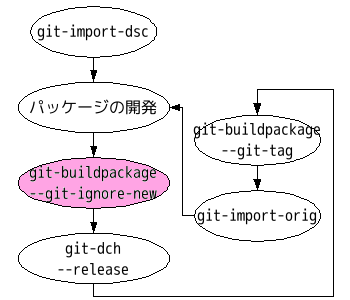
\includegraphics[width=1.0\hsize]{image200804/test1-3.png}
\end{minipage} 
\begin{minipage}{0.45\hsize}

\begin{commandline}
$ git-buildpackage --git-ignore-new\
 -us -uc
\end{commandline}

\end{minipage}
\end{frame}

%%

\begin{frame}[containsverbatim]{パッケージをリリースする}
\begin{minipage}{0.5\hsize}
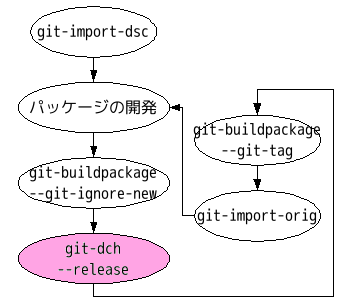
\includegraphics[width=1.0\hsize]{image200804/test1-4.png}
\end{minipage} 
\begin{minipage}{0.45\hsize}
\begin{commandline}
$ git-dch --release
/* エディタが立ち上がり、Debian Changelog 
   を入力する  */
\end{commandline}
\end{minipage}
\end{frame}

\begin{frame}[containsverbatim]{リリースタグを付けて、パッケージを作成する}
\begin{minipage}{0.5\hsize}
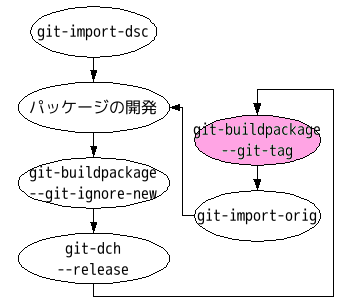
\includegraphics[width=1.0\hsize]{image200804/test1-5.png}
\end{minipage} 
\begin{minipage}{0.45\hsize}
\begin{commandline}
$ git-buildpackage --git-ignore-new\
 --git-tag
$ git tag
debian/1.0.2-1
debian/1.0.2-2
upstream/1.0.2
\end{commandline}
\end{minipage}
\end{frame}

\begin{frame}[containsverbatim]{新しいバージョンにする}
\begin{minipage}{0.5\hsize}
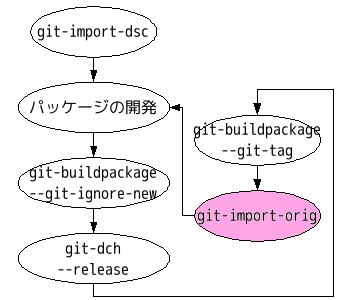
\includegraphics[width=1.0\hsize]{image200804/test1-6.png}
\end{minipage} 
\begin{minipage}{0.45\hsize}
\begin{commandline}
$ git-import-orig /tmp/isight-\
firmware-tools-1.2.tar.gz
Upstream version is 1.2.0
Importing '/tmp/isight-firmware\
-tools-1.2.tar.gz' to branch 'upstream'...
Switched to branch "upstream"
rm 'isight.rules.in'
rm 'po/fr_FR.po'
Created commit f5c85da: Imported\
 Upstream version 1.2.0
 33 files changed, 4434 insertio\
ns(+), 1332 deletions(-)

.......<snip>

 src/udev.c                      \
       |  164 +++
 33 files changed, 4434 insertion\
s(+), 1332 deletions(-)
 rename po/{fr_FR.po => fr.po} (66%)
 create mode 100644 src/50-isight-\
firmware.fdi
\end{commandline}
\end{minipage}
\end{frame}

\begin{frame}[containsverbatim]{新しいバージョンにする}
\begin{minipage}{0.5\hsize}
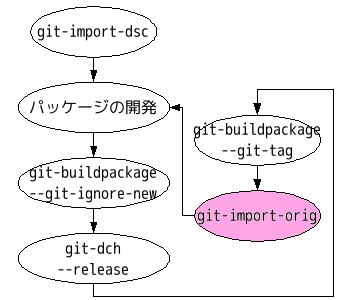
\includegraphics[width=1.0\hsize]{image200804/test1-6.png}
\end{minipage} 
\begin{minipage}{0.45\hsize}
\begin{commandline}
 create mode 100644 src/callout.c
 create mode 100644 src/isight-firm\
ware.fdi
 rename isight.rules.in => src/isigh\
t.rules.in (100%)
 create mode 100644 src/load.h
 create mode 100644 src/udev.c
Succesfully merged version 1.2 of \
/home/iwamatsu/Desktop/isight-firmwar\
e-tools-1.2.tar.gz into .
$ git branch
debian/1.0.2-1
debian/1.0.2-2
upstream/1.0.2
upstream/1.2
$ cat debian/changelog
isight-firmware-tools (1.2-1) unstable;\
 urgency=low

  * New Upstream Version

 -- Nobuhiro Iwamatsu <iwamatsu@\
nigauri.org>  Fri, 11 Apr 2008 17:18:23 +0900

\end{commandline}
\end{minipage}
\end{frame}

\begin{frame}[containsverbatim]{新たにパッケージ化する場合}
\begin{minipage}{0.5\hsize}
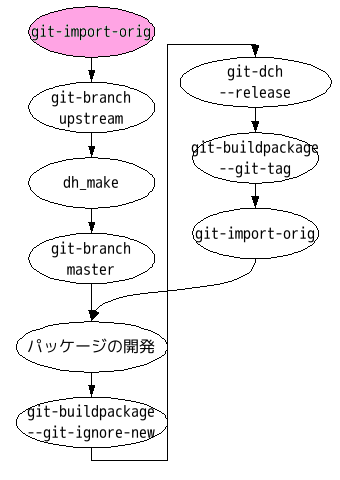
\includegraphics[width=1.0\hsize]{image200804/test-1.png}
\end{minipage} 
\begin{minipage}{0.45\hsize}
\begin{commandline}
$ mkdir isight-firmware-loader-1.2
$ cd isight-firmware-tools-1.2
$ git-init
$ git-import-orig -u 1.2 \
/tmp/isight-firmware-tools-1.2.tar.gz
Upstream version is 1.2
Initial import of '/tmp/isight-\
firmware-tools-1.2.tar.gz' ...
Succesfully merged version 1.2 \
of /tmp/isight-firmware-tools-1.2.tar.gz into .
$ git log
commit 9bf014aee2f834576f8f03d67\
ab66e8c85726832
Author: Nobuhiro Iwamatsu <iwamat\
su@nigauri.org>
Date:   Tue Apr 8 21:42:55 2008 +0900

    Imported Upstream version 1.2
$ git branch
* master
  upstream
$ git tag
upstream/1.2
$ git branch upsteam
$ dh_make
$ git branch master
\end{commandline}

\end{minipage}
\end{frame}


\begin{frame}[containsverbatim]{新たにパッケージ化する場合}
\begin{minipage}{0.5\hsize}
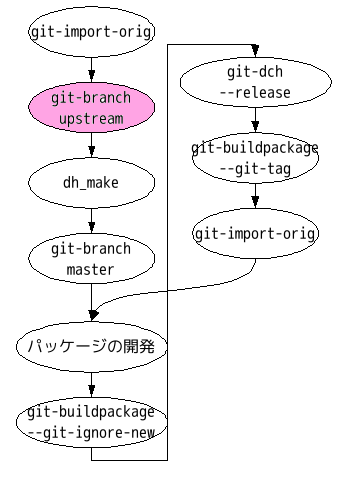
\includegraphics[width=1.0\hsize]{image200804/test-2.png}
\end{minipage} 
\begin{minipage}{0.45\hsize}
\begin{commandline}
$ mkdir isight-firmware-loader-1.2
$ cd isight-firmware-tools-1.2
$ git-init
$ git-import-orig -u 1.2 \
/tmp/isight-firmware-tools-1.2.tar.gz
Upstream version is 1.2
Initial import of '/tmp/isight-\
firmware-tools-1.2.tar.gz' ...
Succesfully merged version 1.2 \
of /tmp/isight-firmware-tools-1.2.tar.gz into .
$ git log
commit 9bf014aee2f834576f8f03d67\
ab66e8c85726832
Author: Nobuhiro Iwamatsu <iwamat\
su@nigauri.org>
Date:   Tue Apr 8 21:42:55 2008 +0900

    Imported Upstream version 1.2
$ git branch
* master
  upstream
$ git tag
upstream/1.2
$ git branch upsteam
$ dh_make
$ git branch master
\end{commandline}

\end{minipage}
\end{frame}


\begin{frame}[containsverbatim]{新たにパッケージ化する場合}
\begin{minipage}{0.5\hsize}
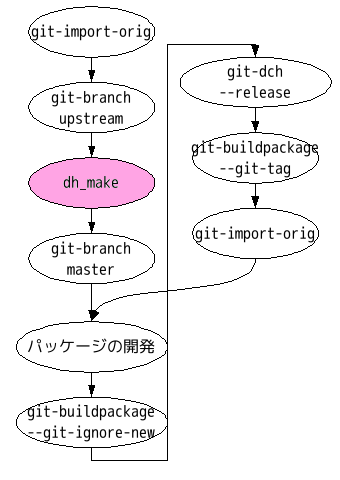
\includegraphics[width=1.0\hsize]{image200804/test-3.png}
\end{minipage} 
\begin{minipage}{0.45\hsize}
\begin{commandline}
$ mkdir isight-firmware-loader-1.2
$ cd isight-firmware-tools-1.2
$ git-init
$ git-import-orig -u 1.2 \
/tmp/isight-firmware-tools-1.2.tar.gz
Upstream version is 1.2
Initial import of '/tmp/isight-\
firmware-tools-1.2.tar.gz' ...
Succesfully merged version 1.2 \
of /tmp/isight-firmware-tools-1.2.tar.gz into .
$ git log
commit 9bf014aee2f834576f8f03d67\
ab66e8c85726832
Author: Nobuhiro Iwamatsu <iwamat\
su@nigauri.org>
Date:   Tue Apr 8 21:42:55 2008 +0900

    Imported Upstream version 1.2
$ git branch
* master
  upstream
$ git tag
upstream/1.2
$ git branch upsteam
$ dh_make
$ git branch master
\end{commandline}

\end{minipage}
\end{frame}



\begin{frame}[containsverbatim]{新たにパッケージ化する場合}
\begin{minipage}{0.5\hsize}
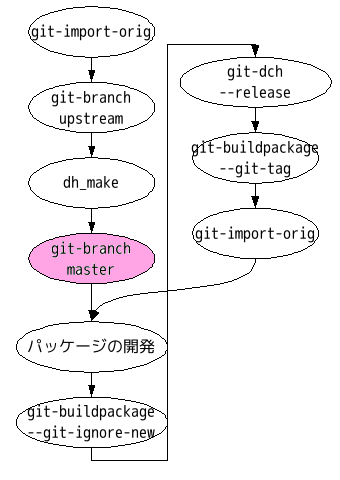
\includegraphics[width=1.0\hsize]{image200804/test-4.png}
\end{minipage} 
\begin{minipage}{0.45\hsize}
\begin{commandline}
$ mkdir isight-firmware-loader-1.2
$ cd isight-firmware-tools-1.2
$ git-init
$ git-import-orig -u 1.2 \
/tmp/isight-firmware-tools-1.2.tar.gz
Upstream version is 1.2
Initial import of '/tmp/isight-\
firmware-tools-1.2.tar.gz' ...
Succesfully merged version 1.2 \
of /tmp/isight-firmware-tools-1.2.tar.gz into .
$ git log
commit 9bf014aee2f834576f8f03d67\
ab66e8c85726832
Author: Nobuhiro Iwamatsu <iwamat\
su@nigauri.org>
Date:   Tue Apr 8 21:42:55 2008 +0900

    Imported Upstream version 1.2
$ git branch
* master
  upstream
$ git tag
upstream/1.2
$ git branch upsteam
$ dh_make
$ git branch master
\end{commandline}

\end{minipage}
\end{frame}



\section{アップストリームの VCS と付き合う}
\emtext{アップストリームの VCS と付き合う}

\begin{frame}[containsverbatim]{アップストリームの VCS と付き合う}

\begin{itemize}
\item アップストリームが VCS を使っている
\item 自分とは趣味の異なるVCSを使っている
\item Debian Package メンテナとしてどのように付き合えばいいのか
\end{itemize}
\end{frame}


\begin{frame}[containsverbatim]{アップストリームが Subversion を使っている場合}

\begin{itemize}
\item 自分も Subversionを使っている場合

svn-buildpackage で連携することが可能

\item Git 使いたい

git-svn で Git リポジトリ形式に変換してから使う

\end{itemize}
\end{frame}


\begin{frame}[containsverbatim]{SVN のリポジトリから Git のリポジトリへ変換する}

\begin{minipage}{0.48\hsize}
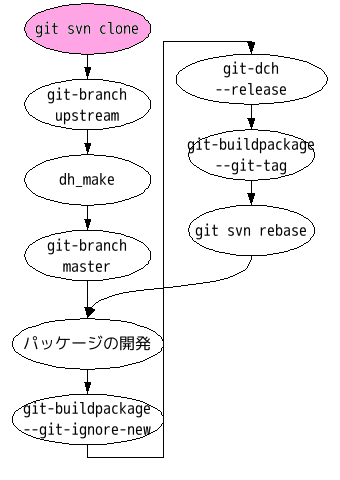
\includegraphics[width=1.0\hsize]{image200804/test2-1.png}
\end{minipage} 
\begin{minipage}{0.45\hsize}
\begin{commandline}
$ mkdir test
$ git svn clone svn://test/trunk test-0.0.1
\end{commandline}
\end{minipage} 
\end{frame}

\begin{frame}[containsverbatim]{取得したコードを元に Debian Package を作成する}
\begin{minipage}{0.48\hsize}
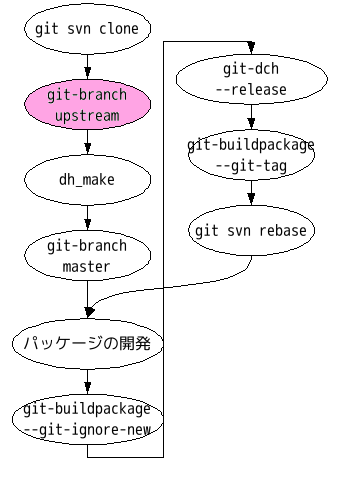
\includegraphics[width=1.0\hsize]{image200804/test2-2.png}
\end{minipage} 
\begin{minipage}{0.45\hsize}
\begin{commandline}
$ git branch
master
$ git branch upstream
$ git checkout upstream
$ git tag upstream/0.0.1
$ dh_make --createorig
$ git branch master
-- Debian Package 用のファイル作成などを行う
$ git-buildpackage -us -uc \
--git-ignore-new
$ debuild clean
$ git add debian
$ git commit -a
$ git-buildpackage -us -uc \
--git-ignore-new --git-tag
\end{commandline}
\end{minipage} 
\end{frame}


\begin{frame}[containsverbatim]{Subversion リポジトリの情報を取得する}
\begin{minipage}{0.48\hsize}
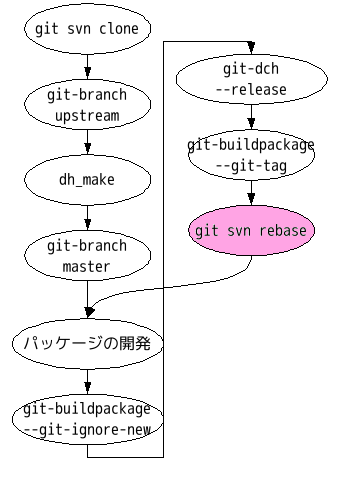
\includegraphics[width=1.0\hsize]{image200804/test2-3.png}
\end{minipage} 
\begin{minipage}{0.45\hsize}
\begin{commandline}
$ git checkout upstream
$ git svn rebase
\end{commandline}
\end{minipage} 
\end{frame}


\begin{frame}[containsverbatim]{すでにあるパッケージと Git リポジトリを元に作成する}

\begin{minipage}{0.48\hsize}
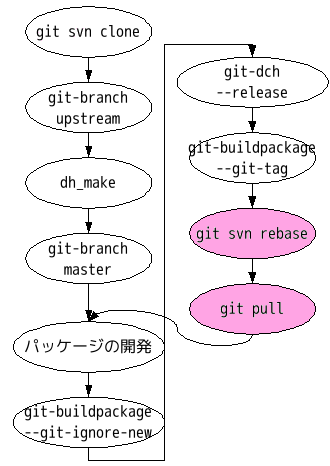
\includegraphics[width=1.0\hsize]{image200804/test3-1.png}
\end{minipage} 
\begin{minipage}{0.45\hsize}
\begin{commandline}

$ git svn clone svn://svn.berlios.de/\
linux-uvc/linux-uvc/trunk\
 linux-uvc.git
$ git import-dsc  ../../../debian/\
linux-uvc_0.1.0.svn193-2.dsc
$ cd linux-uvc
$ git branch
* master
  upstream
$ git tag
debian/0.1.0.svn193-2
upstream/0.1.0.svn193
$ git checkout upstream
$ git pull ../linux-uvc.git/
$ git tag upstream/0.1.0.svn201
$ git checkout master
$ dch -v 0.1.0.svn201
$ git-buildpackage -us -uc \
--git-ignore-new
$ debuild clean
$ git commit -a
$ git-buildpackage -us -us \
--git-ignore-new --git-tag
\end{commandline}
\end{minipage} 
\end{frame}

\begin{frame}{git-svn + git-buildpaclageの問題点}
\begin{itemize}
\item Gitの利点がうまく利用できない

  git svn rebase を使っての開発方法が不明
\item git tag がめんどう。

  Subversion のリリースタグをうまく活用できないか。
\end{itemize}
\end{frame}

\end{document}

;;; Local Variables: ***
;;; outline-regexp: "\\([ 	]*\\\\\\(documentstyle\\|documentclass\\|emtext\\|section\\|begin{frame}\\)\\*?[ 	]*[[{]\\|[]+\\)" ***
;;; End: ***
